\section{Ken Lee}
\subsection{intro}
I am a first year PhD student under Dr. Brown.  
We have discussed several ideas, and I have a list of conferences and journals that he publishes to most often for reference.
I am really enjoying the material in this class, though I really have to change habits so that I can spend blocks of time reading papers that I may eventually use.  
Even more import to me, is the information that I gain from the papers to stay current in my field.
Besides school and working fulltime, I enjoy sailing as my hobby to really unwind.  
Below is a picture of me at the helm of our 19 ft Flying Scot sailboat named Fin and Tonic.
\begin{figure}[!htb]
\centering
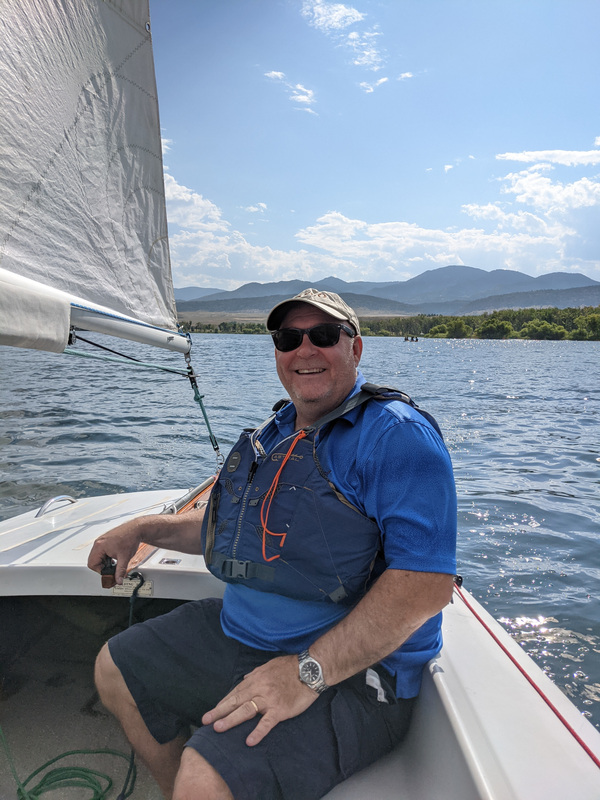
\includegraphics[width=0.5\textwidth]{sailing_flyingscot.jpg}
\end{figure}

\subsection{git repo}
\url{https://github.com/kalee/Schelling-Segregation.git} This is a project that I worked on in another class.  
It is Java code that runs the Shelling Segregation model.  
This is related to my field of research in that it is using agents that work locally towards a specific goal.  
A goal that wasn't worked on was worst-case analysis.  
We setup a boundary of a maximum of 100x100 grid squares.  
Much larger, and it really takes a long time to complete.  
There is a lot of code to run
through, and determining $\Theta$ for worst case was not the point, though could be included.

\subsection{Questions}
\textbf{Question 1:} Hey Ken! How did you decide to study at UCCS?\\
I have a son who is graduating from UCCS this December with a BS with I believe is a triple major (EE, Mathematics, and Computer Science).  I'm obviously pretty proud of his accomplishments.  Well, a few years ago, I was taking C Programming at ACC.  I was not really happy with what I got out of it.  I did really like the price, but it just wasn't worth it to me.  I talked to my son, and he mentioned some of the classes in CS and a some of the work he was doing.  I was sold at that point.  I started with 1450, then jumped up to 5720.  I talked to my professor about what I wanted to accomplish, which is really solving problems, and discussed the PhD program and how that would help me to attain my goals.  That is the short version, but is how I decided to study at UCCS.\\

